A permanent magnet with magnetisation vector \(\mathbf{M}\) can be modelled as a collection of magnetic charges described by the magnetic charge model \cite{Furlani2001}. The magnetic field \(\mathbf{B}\) at a point in space outside the magnet \(\mathbf{x}\) can be calculated using the charge model given by

\begin{equation}
\label{eqn:p2chargemodel}
\mathbf{B}\left( \mathbf{x} \right) = \frac{\mu_0}{4\pi} \left( \oint_{S} \left( \mathbf{M} \cdot \hat{\mathbf{n}} \right) \frac{\mathbf{x} - \mathbf{x}'}{\left| \mathbf{x} - \mathbf{x}' \right|^3} \ ds' - \int_{V} \left( \nabla \cdot \mathbf{M} \right) \frac{\mathbf{x} - \mathbf{x}'}{\left| \mathbf{x} - \mathbf{x}' \right|^3} \ dv' \right) \text{,}
\end{equation}

\noindent where \(\mu_0\) is the permeability of free space, \(V\) is the magnet volume, \(S\) is the magnet surface, \(\mathbf{x}'\) is a point in or on the magnet, and \(\hat{\mathbf{n}} = \left[ n_x, n_y, n_z \right]\) is the outward-facing unit normal vector of the magnet surface. If the magnet is assumed ideal; that is, the magnetisation \(\mathbf{M}\) is assumed uniform and constant and the relative permeability is assumed unity, the volume integral disappears as \(\nabla \cdot \mathbf{M} = 0\), leaving only the surface integral

\begin{equation}
\label{eqn:p2chargeB}
\mathbf{B}\left( \mathbf{x} \right) = \frac{\mu_0}{4\pi} \oint_{S} \left( \mathbf{M} \cdot \hat{\mathbf{n}} \right) \frac{\mathbf{x} - \mathbf{x}'}{\left| \mathbf{x} - \mathbf{x}' \right|^3} \ ds' \text{.}
\end{equation}

\noindent Equation (\ref{eqn:p2chargeB}) implies the magnet can be considered a set of \(n\) magnetically charged surfaces \(S_{\!i}\), with the total field given by

\begin{equation}
\label{eqn:p2chargeBdiscrete}
\mathbf{B}\left( \mathbf{x} \right) = \sum_{i=1}^n \frac{\mu_0}{4\pi} \int_{S_i} \left( \mathbf{M} \cdot \hat{\mathbf{n}}_i \right) \frac{\mathbf{x} - \mathbf{x}'}{\left| \mathbf{x} - \mathbf{x}' \right|^3} \ ds_i' = \sum_{i=1}^n \textbf{B}_i\left(\textbf{x}\right) \text{,}
\end{equation}

\noindent where \(\textbf{B}_i\left(\mathbf{x}\right)\) is the magnetic field contribution of the surface \(S_{\!i}\).

The total magnetic field due to the magnet can be found by solving Equation (\ref{eqn:p2chargeBdiscrete}), i.e., summing the field contributions from each surface \(S_{\!i}\) to give the total magnetic field. To do this, first the polyhedral magnet must be decomposed into a set of charged surfaces, as described in the following section.

\subsection{Polyhedral decomposition}\label{sec:p2polyhedrondecomposition}

To calculate the magnetic field at a point \(\mathbf{x} = \left[ x, y, z\right]\) due to a polyhedral permanent magnet with surface \(S\), the magnet is considered a collection of polygonal surfaces \(S_{\!i}\). The field calculation begins by considering one polygonal surface \(S_{\!i}\) with magnetic charge density \(\mathbf{M} \cdot \hat{\mathbf{n}}_i\), where \(\hat{\mathbf{n}}_i\) is the outward-facing unit normal vector of the surface \(S_{\!i}\). This surface and the point \(\mathbf{x}\) are rotated in 3D space about the origin such that \(S_{\!i}\) is parallel to the \(XY\)-plane; that is, \(S_{\!i}\) is rotated such that its normal vector is parallel to the \(z\)-axis. This is done by postmultiplying \(\mathbf{x}\) and each vertex of \(S_{\!i}\) by the rotation matrix \(R\), given by

\begin{equation}
R = \begin{bmatrix}
m & 0 & n_x \\[4pt]
-n_xn_y/m & n_z/m & n_y \\[4pt]
-n_xn_z/m & -n_y/m & n_z
\end{bmatrix} \text{,}
\end{equation}

\noindent where \(m = \sqrt{n_y^2+n_z^2}\). A full derivation of \(R\) is given in \ref{sec:p2Rderivation}. Note that if \(\hat{\mathbf{n}}_i = \left[\pm1,0,0\right]\), then the surface is parallel to the \(YZ\) plane and \(n_y = n_z = 0 \implies m = 0\) and \(R\) is undefined. In this case, the limit as \(n_z\) approaches 0 from the positive side is taken and \(R\) should instead be defined as

\begin{equation}
R = \begin{bmatrix}
\phantom{-}0 & 0 & 1 \\
\phantom{-}0 & 1 & 0 \\
-1 & 0 & 0 \end{bmatrix} \text{.}
\end{equation}

After rotation, the point at which the field is to be computed is given by \(\mathbf{x}_r = \mathbf{x}R\) and the surface \(S_{\!i}\) is parallel to the \(XY\)-plane. Lines are drawn through each vertex of the polygonal surface parallel to the \(y\)-axis, dividing the polygon into a series of trapezia \(T_{\!j}\), as shown in Figure \ref{fig:p2polyhedrondecomposition}. Note that for this work, a triangle is considered a degenerate case of a trapezium with one of the parallel sides having a length of zero. The magnetic field contribution of each trapezium is computed using the solution to Equation (\ref{eqn:p2chargeB}) described in Section \ref{sec:p2fieldcalc}.
\begin{figure}[h]
	\centering
	\begin{subfigure}{0.6\textwidth}
	\centering
	\begin{tikzpicture}[scale=2.5]
		\coordinate(c1) at (-0.47943,0.87758);
		\coordinate(c2) at (-0.98278,-0.18477);
		\coordinate(c3) at (-0.12797,-0.99178);
		\coordinate(c4) at (0.90369,-0.42818);
		\coordinate(c5) at (0.68648,0.72715);
	\draw (c1) -- (c2) -- (c3) -- (c4) -- (c5) -- cycle;
		\draw[->] (-1.2,-1.3) -- (-0.2,-1.3);
		\draw[->] (-1.2,-1.3) -- (-1.2,-0.3);		\node(x) at (-0.1,-1.3) {\(x\)};
		\node(y) at (-1.2,-0.2) {\(y\)};
		
		\node(Si) at (0,0) {\(S_i\)};
	\end{tikzpicture}
	\caption{}\label{fig:p2polyhedrondecompositiona}
\end{subfigure}

\vspace{40pt}

\begin{subfigure}{0.6\textwidth}
	\centering
	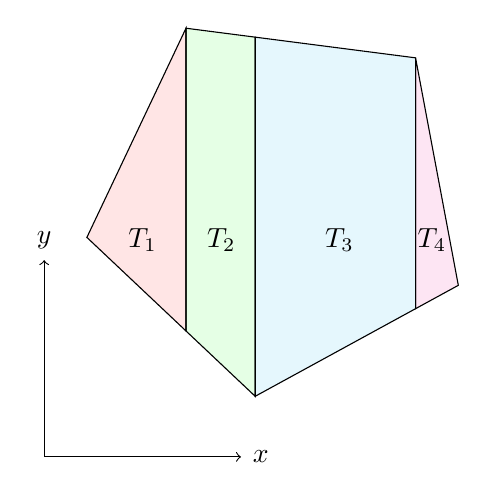
\begin{tikzpicture}[scale=2.5]
		\coordinate(c1) at (-0.98278,-0.18477);
		\coordinate(c2) at (-0.98278,-0.18477);
		\coordinate(c3) at (-0.47943,0.87758);
		\coordinate(c4) at (-0.47943,-0.65998);
		\filldraw[fill=red, fill opacity=0.1] (c1) -- (c2) -- (c3) -- (c4) -- cycle;
		\coordinate(c5) at (-0.47943,-0.65998);
		\coordinate(c6) at (-0.47943,0.87758);
		\coordinate(c7) at (-0.12797,0.83224);
		\coordinate(c8) at (-0.12797,-0.99178);
		\filldraw[fill=green, fill opacity=0.1] (c5) -- (c6) -- (c7) -- (c8) -- cycle;
		\coordinate(c9) at (-0.12797,-0.99178);
		\coordinate(c10) at (-0.12797,0.83224);
		\coordinate(c11) at (0.68648,0.72715);
		\coordinate(c12) at (0.68648,-0.54684);
		\filldraw[fill=cyan, fill opacity=0.1] (c9) -- (c10) -- (c11) -- (c12) -- cycle;
		\coordinate(c13) at (0.68648,-0.54684);
		\coordinate(c14) at (0.68648,0.72715);
		\coordinate(c15) at (0.90369,-0.42818);
		\coordinate(c16) at (0.90369,-0.42818);
		\filldraw[fill=magenta, fill opacity=0.1] (c13) -- (c14) -- (c15) -- (c16) -- cycle;
		\draw[->] (-1.2,-1.3) -- (-0.2,-1.3);
		\draw[->] (-1.2,-1.3) -- (-1.2,-0.3);		\node(x) at (-0.1,-1.3) {\(x\)};
		\node(y) at (-1.2,-0.2) {\(y\)};
		
		% Label trapezia
		\node(t1) at (-0.7,-0.2) {\(T_1\)};
		\node(t2) at (-0.3,-0.2) {\(T_2\)};
		\node(t3) at (0.3,-0.2) {\(T_3\)};
		\node(t4) at (0.77,-0.2) {\(T_4\)};
	\end{tikzpicture}
	\caption{}\label{fig:p2polyhedrondecompositionb}
\end{subfigure}

	\caption{After the polygonal surface \(S_{\!i}\) has been rotated such that it is parallel to the \(XY\)-plane (\subref{fig:p2polyhedrondecompositiona}), lines are drawn through each vertex parallel to the \(y\)-axis, dividing the polygon into trapezia (\subref{fig:p2polyhedrondecompositionb}).}
	\label{fig:p2polyhedrondecomposition}
\end{figure}

\subsection{Magnetic field calculation of charged trapezia}\label{sec:p2fieldcalc}

\begin{figure}
	\centering
	\def\lim{10}

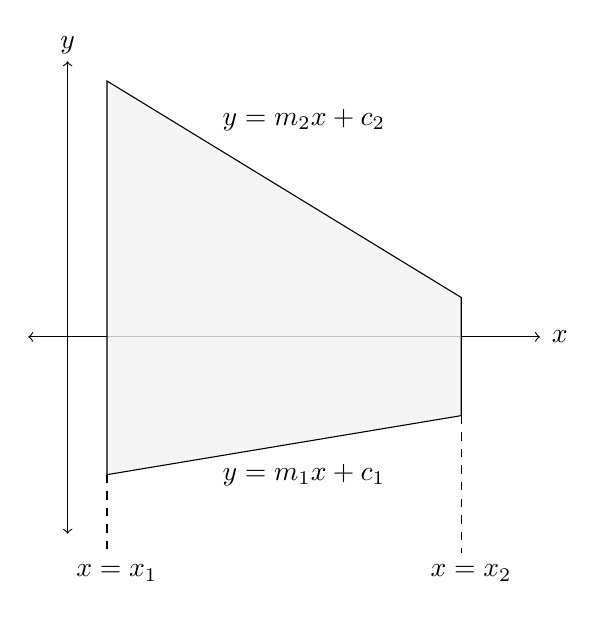
\begin{tikzpicture}[scale=0.5]
	\coordinate(negx) at (-1,0);
	\coordinate(posx) at (\lim+2,0);
	\coordinate(negy) at (0,-5);
	\coordinate(posy) at (0,7);
	
	\coordinate(TL) at (1,6.5);
	\coordinate(BL) at (1,-3.5);
	\coordinate(TR) at (\lim,1);
	\coordinate(BR) at (\lim,-2);
	
	\draw[<->] (negx) -- (posx);
	\draw[<->] (negy) -- (posy);
	\filldraw[fill=black!5, fill opacity=0.8] (BL) -- (BR) -- (TR) -- (TL) -- cycle;
	
	\draw[dashed] (BL) -- (1,-5.5);
	\node(x1) at (1.25,-6) {\(x = x_1\)};
	\draw[dashed] (BR) -- (\lim,-5.5);
	\node(x2) at (\lim+0.25,-6) {\(x = x_2\)};
	\node(m1c1) at (6,-3.5) {\(y=m_1x+c_1\)};
	\node(m2c2) at (6,5.5) {\(y=m_2x+c_2\)};
	\node(x) at (\lim+2.5,0) {\(x\)};
	\node(y) at (0,7.4) {\(y\)};
\end{tikzpicture}
	\caption{A magnetically charged trapezial surface. It is parallel to the \(XY\)-plane with \(z\)-coordinate \(z = z'\) and a pair of opposite edges parallel to the \(y\)-axis.}
	\label{fig:p2trapezium}
\end{figure}

Given a magnetically charged trapezium parallel to the \(XY\)-plane at \(z = z'\), with the parallel lines having equations \(x = x_1\) and \(x = x_2\) and the non-parallel lines having equations \mbox{\(y = m_1x+c_1\)} and \mbox{\(y = m_2x+c_2\)} (shown in Figure \ref{fig:p2trapezium}), the magnetic field contribution \(\left[B_{xj},B_{yj},B_{zj}\right]\) at a point \(\mathbf{x}_r = \left[ x_r, y_r, z_r \right]\) is given by

\begin{equation}
	\label{eqn:p2myintegral}
	\left[ B_{xj}, B_{yj}, B_{zj} \right] = \frac{\mu_0}{4\pi} \int_{x_1}^{x_2} \int_{m_1x'+c_1}^{m_2x'+c_2} \left( \mathbf{M} \cdot \hat{\mathbf{n}} \right) \left[ I_x, I_y, I_z \right] \ dy' \ dx'
\end{equation}

\noindent where

\begin{align}
	I_x &= \frac{\left[x_r-x'\right]}{\left(\left(x_r-x'\right)^2+\left(y_r-y'\right)^2+\left(z_r-z'\right)^2\right)^{3/2}} \text{,} \nonumber \\
	I_y &=  \frac{\left[y_r-y'\right]}{\left(\left(x_r-x'\right)^2+\left(y_r-y'\right)^2+\left(z_r-z'\right)^2\right)^{3/2}} \text{,} \\
	I_z &=  \frac{\left[z_r-z'\right]}{\left(\left(x_r-x'\right)^2+\left(y_r-y'\right)^2+\left(z_r-z'\right)^2\right)^{3/2}} \text{.} \nonumber
\end{align}

After solving this difficult integral and simplifying the result\footnote{The full derivation for this solution is outlined in Appendix \ref{app:fieldEquations}}, the authors derived the following solution to Equation (\ref{eqn:p2myintegral}).

\begin{align}\label{eqn:p2fieldequation}
\begin{split}
B_{xj} &= \frac{\mu_0}{4\pi} \left(\mathbf{M} \cdot \hat{\mathbf{n}}\right) \sum_{p=1}^2 \sum_{q=1}^2 \left[ \left( -1 \right) ^{p+q} \left( \ln \left( T_{pq} \right) - \frac{m_p}{\sqrt{1+m_p^2}} \ln \left(S_{\!pq}\right) \right) \right] \\
B_{yj} &= \frac{\mu_0}{4\pi} \left(\mathbf{M} \cdot \hat{\mathbf{n}}\right) \sum_{p=1}^2 \sum_{q=1}^2 \left[ \left( -1 \right)^{p+q} \frac{1}{\sqrt{1+m_p^2}} \ln \left( S_{\!pq} \right) \right] \\
B_{zj} &= \frac{\mu_0}{4\pi} \left(\mathbf{M} \cdot \hat{\mathbf{n}}\right) \sum_{p=1}^2 \sum_{q=1}^2 \Bigg[ \left( -1 \right) ^{p+q} \arctan \left( U_{pq} \right) \Bigg] \text{,}
\end{split}
\end{align}

\noindent with

\begin{align}\label{eqn:p2intermediatevars}
\begin{split}
X &= x_q - x_r \\
Y &= c_p + m_px_q - y_r \\
Z &= z' - z_r \\
R_{pq} &= \sqrt{X^2 + Y^2 + Z^2} \\
S_{\!pq} &= X + m_pY + \sqrt{1+m_p^2}R_{pq} \\
T_{pq} &= R_{pq} + Y \\
U_{pq} &= \frac{m_p\left(X^2+Z^2\right)-XY}{ZR_{pq}} \text{.}
\end{split}
\end{align}

Equation (\ref{eqn:p2fieldequation}) describes the magnetic field produced by the magnetically charged trapezium shown in Figure \ref{fig:p2trapezium}. Further processing is required to calculate the magnetic field produced by a polyhedral magnet, as described in the following sections.

\subsubsection{Special case when \(m_p = 0\)}

Equation (\ref{eqn:p2fieldequation}) can be applied to a cuboidal magnet by using six rectangular faces with \(m_p = 0\) for all \(p\). Substituting \(m_p = 0\) into Equations (\ref{eqn:p2fieldequation}) and (\ref{eqn:p2intermediatevars}) gives the following simplified equations for a cuboidal magnet.

\begin{align}\label{eqn:p2cuboidequation}
\begin{split}
B_x &= \frac{\mu_0}{4\pi} \left(\mathbf{M} \cdot \hat{\mathbf{n}}\right) \sum_{p=1}^2 \sum_{q=1}^2 \left[ \left( -1 \right) ^{p+q} \ln \left( T_{pq} \right) \right] \\
B_y &= \frac{\mu_0}{4\pi} \left(\mathbf{M} \cdot \hat{\mathbf{n}}\right) \sum_{p=1}^2 \sum_{q=1}^2 \left[ \left( -1 \right) ^{p+q} \ln \left( S_{\!pq} \right) \right] \\
B_z &= \frac{\mu_0}{4\pi} \left(\mathbf{M} \cdot \hat{\mathbf{n}}\right) \sum_{p=1}^2 \sum_{q=1}^2 \left[ \left( -1 \right) ^{p+q} \arctan \left( U_{pq} \right) \right] \text{,}
\end{split}
\end{align}

\noindent with

\begin{align}\label{eqn:p2cuboidvars}
\begin{split}
X &= x_q - x_r \\
Y &= c_p - y_r \\
Z &= z' - z_r \\
R_{pq} &= \sqrt{X^2 + Y^2 + Z^2} \\
S_{\!pq} &= X + R_{pq} \\
T_{pq} &= R_{pq} + Y \\
U_{pq} &= \frac{-XY}{ZR_{pq}} \text{.}
\end{split}
\end{align}

It can be shown that these equations are equivalent to those published by \textcite{Akoun1984}, \textcite{Bancel1999}, and \textcite{Ravaud2009}, verifying Equation (\ref{eqn:p2fieldequation}) for cuboidal magnets\footnote{The equations in \cite{Akoun1984}, \cite{Bancel1999}, and \cite{Ravaud2009} are of the same form, but with different variable names.}.

\subsection{Polyhedral recomposition}

Once the magnetic field contributions from each trapezium \(T_{\!j}\) is computed, all contributions are summed to give the total field due to the polygonal surface \(S_{\!i}\),

\begin{equation}
\begin{bmatrix}
B_{xi} & B_{yi} & B_{zi}
\end{bmatrix} = \sum_j \begin{bmatrix}
B_{xj} & B_{yj} & B_{zj} \end{bmatrix} \text{.}
\end{equation}

\noindent This magnetic field vector is then postmultiplied by \(R^\text{T}\) to give the field due to \(S_{\!i}\) in the original coordinate system,

\begin{equation}
\textbf{B}_i\left(\textbf{x}\right) = \begin{bmatrix}
B_{xi} & B_{yi} & B_{zi} \end{bmatrix}
R^\textsf{T} \text{,}
\end{equation}

\noindent where \(R^{\textsf{T}}\) is the transpose of \(R\).

This process is repeated for each face of the polyhedron. Finally, the field contributions from each polygonal face \(S_{\!i}\) are summed to give the total magnetic field at the point \(\mathbf{x}\) due to the polyhedral permanent magnet,

\begin{equation}
\textbf{B}\left(\textbf{x}\right) = \sum_{i=1}^n \textbf{B}_i\left(\textbf{x}\right) \text{.}
\end{equation}

\subsection{Singularity treatment}

Singularities can be found in Equation (\ref{eqn:p2fieldequation}) when \(S_{\!pq} = 0\), when \(T_{pq} = 0\), or when \(U_{pq} = 0/0\). The regions in which each of these singularities occur are shown in Figure \ref{fig:p2singularities}. Under these conditions, the magnetic field given by Equation (\ref{eqn:p2fieldequation}) is undefined, so these singularities must be resolved to give a robust magnetic field solution.

\begin{figure}
	\centering
	\def\myscale{0.3}
\def\greythick{50}

\begin{subfigure}{0.45\textwidth}
\centering
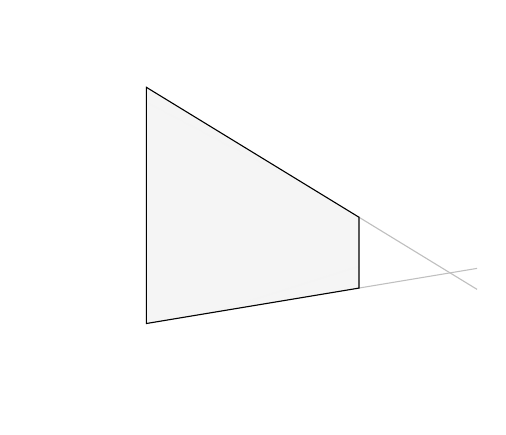
\begin{tikzpicture}[scale=\myscale]
	\coordinate(TL) at (1,6.5);
	\coordinate(BL) at (1,-3.5);
	\coordinate(TR) at (10,1);
	\coordinate(BR) at (10,-2);
	
	% Draw some white lines to make sure all figures are the same size:
	\draw[white] (-4,8.5) -- (15,-1.5);
	\draw[white] (-4,-5.5) -- (15,0.5);
	\draw[white] (1,-7) -- (1,9);
	\draw[white] (11,-7) -- (11,9);
	
	% Draw the singular regions:
	\draw[gray!\greythick] (10,1) -- (15,-2.05555556);
	\draw[gray!\greythick] (10,-2) -- (15,-1.16666667);
	
	% Draw the trapezium:
	\filldraw[fill=black!5, fill opacity=0.8] (BL) -- (BR) -- (TR) -- (TL) -- cycle;
\end{tikzpicture}
\caption{}\label{fig:p2singularitiesa}
\end{subfigure}
\begin{subfigure}{0.45\textwidth}
\centering
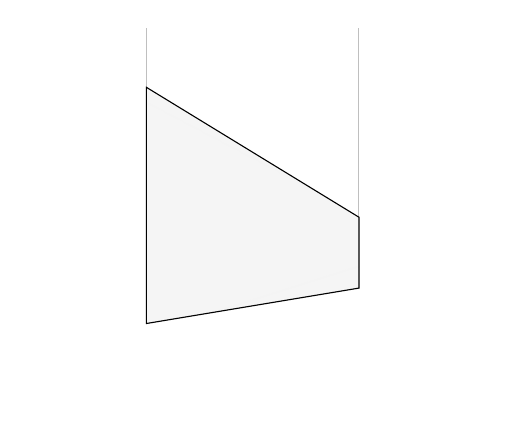
\begin{tikzpicture}[scale=\myscale]
    \coordinate(TL) at (1,6.5);
    \coordinate(BL) at (1,-3.5);
    \coordinate(TR) at (10,1);
    \coordinate(BR) at (10,-2);
	
	% Draw some white lines to make sure all figures are the same size:
	\draw[white] (-4,8.5) -- (15,-1.5);
	\draw[white] (-4,-5.5) -- (15,0.5);
	\draw[white] (1,-7) -- (1,9);
	\draw[white] (11,-7) -- (11,9);
	
	% Draw the singular regions:
	\draw[gray!\greythick] (1,6.5) -- (1,9);
	\draw[gray!\greythick] (10,1) -- (10,9);
	
	% Draw the trapezium:
	\filldraw[fill=black!5, fill opacity=0.8] (BL) -- (BR) -- (TR) -- (TL) -- cycle;
\end{tikzpicture}
\caption{}\label{fig:p2singularitiesb}
\end{subfigure}
\begin{subfigure}{0.45\textwidth}
    \centering
    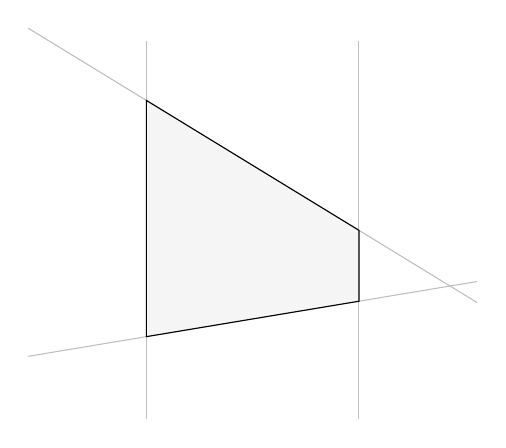
\begin{tikzpicture}[scale=\myscale]
    \coordinate(TL) at (1,6.5);
    \coordinate(BL) at (1,-3.5);
    \coordinate(TR) at (10,1);
    \coordinate(BR) at (10,-2);
	
	% Draw the singular regions:
	\draw[gray!\greythick] (-4,9.55555556) -- (15,-2.05555556);
	\draw[gray!\greythick] (-4,-4.33333333) -- (15,-1.16666667);
	\draw[gray!\greythick] (1,-7) -- (1,9);
	\draw[gray!\greythick] (10,-7) -- (10,9);
	
	% Draw the trapezium:
	\filldraw[fill=black!5, fill opacity=0.8] (BL) -- (BR) -- (TR) -- (TL) -- cycle;
\end{tikzpicture}
\caption{}\label{fig:p2singularitiesc}
\end{subfigure}


	\caption{The regions around a trapezium in which singularities occur. \(S_{\!pq} = 0\) along the grey lines in (\subref{fig:p2singularitiesa}), \(T_{pq} = 0\) along the grey lines in (\subref{fig:p2singularitiesb}), and \(U_{pq} = 0/0\) along the grey lines in (\subref{fig:p2singularitiesc}).}
	\label{fig:p2singularities}
\end{figure}

\subsubsection{Solving \(S_{\!pq} = 0\)}

Substituting \(S_{\!pq} = 0\) into Equation (\ref{eqn:p2intermediatevars}) implies that \(X < 0\), \(Y = m_pX\), and \(Z = 0\). Therefore, any point inline with one of the non-parallel edges and to the right of any trapezium, shown in Figure \ref{fig:p2singularitiesa}, will lead to a singularity in the equations. This can be solved by applying L'H\^{o}pital's rule twice, giving Equation (\ref{eqn:p2Ssingsol}).

When evaluating Equations (\ref{eqn:p2fieldequation}) and (\ref{eqn:p2intermediatevars}), if for any pair \(\left(p,q\right)\), \(X < 0\), \(Y = m_pX\), and \(Z = 0\), this singularity is solved by the redefinition

\begin{equation}\label{eqn:p2Ssingsol}
S_{\!pq} = \frac{1}{R_{pq}} \text{.}
\end{equation}

\subsubsection{Solving \(T_{pq} = 0\)}

Substituting \(T_{pq} = 0\) into Equation (\ref{eqn:p2intermediatevars}) implies that \(X = 0\), \(Y < 0\), and \(Z = 0\). Therefore, if a point is inline with one of the parallel edges of any trapezium and above it, shown in Figure \ref{fig:p2singularitiesb}, a singularity will occur. This can be solved by again applying L'H\^{o}pital's rule twice, giving Equation (\ref{eqn:p2Tsingsol}).

When evaluating Equations (\ref{eqn:p2fieldequation}) and (\ref{eqn:p2intermediatevars}), if for any pair \(\left(p,q\right)\), \(X = Z = 0\) and \(Y < 0\), this singularity is solved by the redefinition

\begin{equation}\label{eqn:p2Tsingsol}
T_{pq} = \frac{1}{R_{pq}} \text{.}
\end{equation}

\subsubsection{Solving \(U_{pq} = 0/0\)}

Setting the denominator of \(U_{pq}\) to 0 in Equation (\ref{eqn:p2intermediatevars}) gives \(Z = 0\) since \(R_{pq} > 0\) for any point not coincident with a vertex. If \(Z = 0\), then the numerator of \(U_{pq}\) also goes to 0 when either \(X = 0\) or \(Y = m_pX\). Therefore, this singularity occurs when \(Z = X = 0\), or when \(Z = Y - m_pX = 0\). The singular regions are shown in Figure \ref{fig:p2singularitiesc}.

Solving the former case, \(X = Z = 0\), requires the use of L'H\^{o}pital's rule once, giving \(U_{pq} = \sgn\left(Y\right)\). However, due to the summation over \(p\) and the term \(\left(-1\right)^{p+q}\) in Equation (\ref{eqn:p2fieldequation}), \(U_{pq}\) can simply be set to 0.

The latter case, namely, \(Z = Y - m_pX = 0\), has a more trivial solution. Since \(Y = m_pX\), the numerator simplifies to \(-m_pZ^2\), leaving \(U_{pq} = -m_pZ/R_{pq}\). Since \(Z = 0\) and \(R_{pq} > 0\), this becomes \(U_{pq} = 0\). These two results give Equation (\ref{eqn:p2Usingsol}).

When evaluating Equations (\ref{eqn:p2fieldequation}) and (\ref{eqn:p2intermediatevars}), if for any pair \(\left(p,q\right)\), \(Z = X = 0\) or \(Z = Y-mX = 0\), this singularity is solved by the redefinition

\begin{equation}\label{eqn:p2Usingsol}
U_{pq} = 0 \text{.}
\end{equation}

\subsection{Computational considerations}

In contrast with previous solutions \cite{Rubeck2013,OConnell2020}, the solution formulated in this paper has been derived to allow the computation of a matrix of points \(P\) to be evaluated with only a single polyhedral decomposition and rotation routine. If \(n\) points are defined as \(\left[x_1, y_1, z_1\right], \dotsc, \left[x_n, y_n, z_n\right]\), then \(P\) is defined by the \(\left( n \times 3\right)\) matrix

\begin{equation}
P = \begin{bmatrix}
x_1 & y_1 & z_1 \\
\vdots & \vdots & \vdots \\
x_n & y_n & z_n
\end{bmatrix} \text{.}
\end{equation}

For a given polygonal facet \(S_{\!i}\) with associated rotation matrix \(R\), \(P_r = PR\) gives a list of rotated points at which the magnetic field can be calculated. Equation (\ref{eqn:p2fieldequation}) is applied to each row of \(P_r\), and the magnetic field components rotated back to the original coordinate system after the computation of the field at all points in \(P_r\). In this way, polyhedron decomposition occurs only once, independent of the number of points, therefore reducing overhead and increasing efficiency.

Using this methodology on a polyhedron with \(E\) edges and \(F\) faces, a maximum of \(2E - F\) trapezia are required (see \ref{sec:p2numtrap}), giving an upper bound on the number of calculations required. If the magnetic field is to be evaluated at \(n\) points, then Equation (\ref{eqn:p2fieldequation}) must be computed a total of up to \(n\left(2E-F\right)\) times with up to \(2F\) total rotations. Therefore, if each computation of Equation (\ref{eqn:p2fieldequation}) takes \(t_n\) seconds and the average overhead for each calculation is \(t_o\), an upper bound for the total expected calculation time is

\begin{equation}
t_{\text{expected}} \leq \left(2E-F\right)\left(t_o + nt_n \right) \text{.}
\end{equation}

\noindent This equation shows that the calculation time scales approximately linearly with the number of points at which the field is calculated.

This methodology was implemented in vectorised Matlab code without parallelisation in Matlab R2017b (MathWorks, Inc., Natick, MA, USA). This was run on a workstation PC with an Intel Xeon E3-1240 v5 at 3.50GHz and 16GB of memory using Windows 10 Enterprise. In an effort to approximate the constants \(t_o\) and \(t_n\), a randomly generated polyhedron was defined, and the magnetic field calculated at a large number of points near the polyhedron. On this particular computer hardware, \(t_o\) was in the order of several milliseconds (\(10^{-3}\) seconds) and \(t_n\) was in the order of several hundred nanoseconds (\(10^{-7}\) seconds). These values will vary when using different computer hardware and software, but the constants stated here give an approximation of calculation time before the algorithm is executed.

This methodology excels when calculating the magnetic field at a large number of points. This is because the rotation and decomposition routines are the slowest parts of the algorithm, but only occur once, no matter the number of field calculations. The computation of Equation (\ref{eqn:p2fieldequation}) is orders of magnitude faster than the rotation and decomposition routine, and thus a larger number of field calculations has little effect on the computation time.

The Matlab implementation of the algorithm presented in this paper is available as the file polyhedronField.m at

\noindent \url{github.com/jlgO'Connell/polyhedralMagnet}.
